\documentclass[titlepage]{article}

\usepackage{graphicx}
\usepackage{blindtext}
\usepackage{wrapfig}

\author{Sam Leonard}
\title{Test Document}
\date{}

\begin{document}

\maketitle

\section{Introduction}

This is a bunch of text.
This is more text.

This is referring to section \ref{examples}

need two enters to actually indent to another line
\subsection{This is a subsection\label{examples}}

\textbf{This is bold text.}

\textit{This is italic text.}

\emph{This is emphatic text.}

\underline{This is underlined text.}

``This is in quotes''

this refers to item\ref{bbb} of list\ref{lists}

\subsubsection{This is a subsubsection with some lists}

\begin{enumerate}\label{lists}
  \item item 1
  \item wow this is cool
  \item wow now this is item 3
  \item woosh\label{bbb}

\end{enumerate}

\begin{itemize}

  \item this is an itemized list
  \item wowowo
  \item bananana

\end{itemize}

\section{Images}

\blindtext

\begin{center}
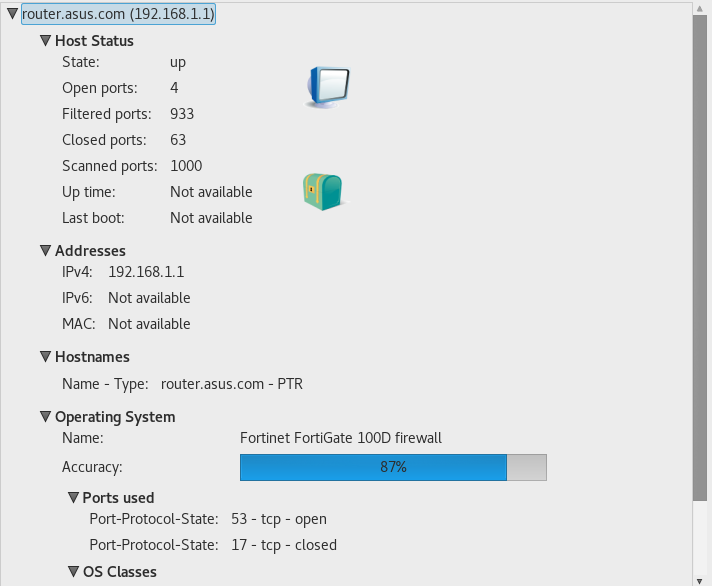
\includegraphics[width=\textwidth]{router_OS_scan.png}
\end{center}

\blindtext

below you can see a fully working SYN scan.

\begin{figure}[h]
  \centering
  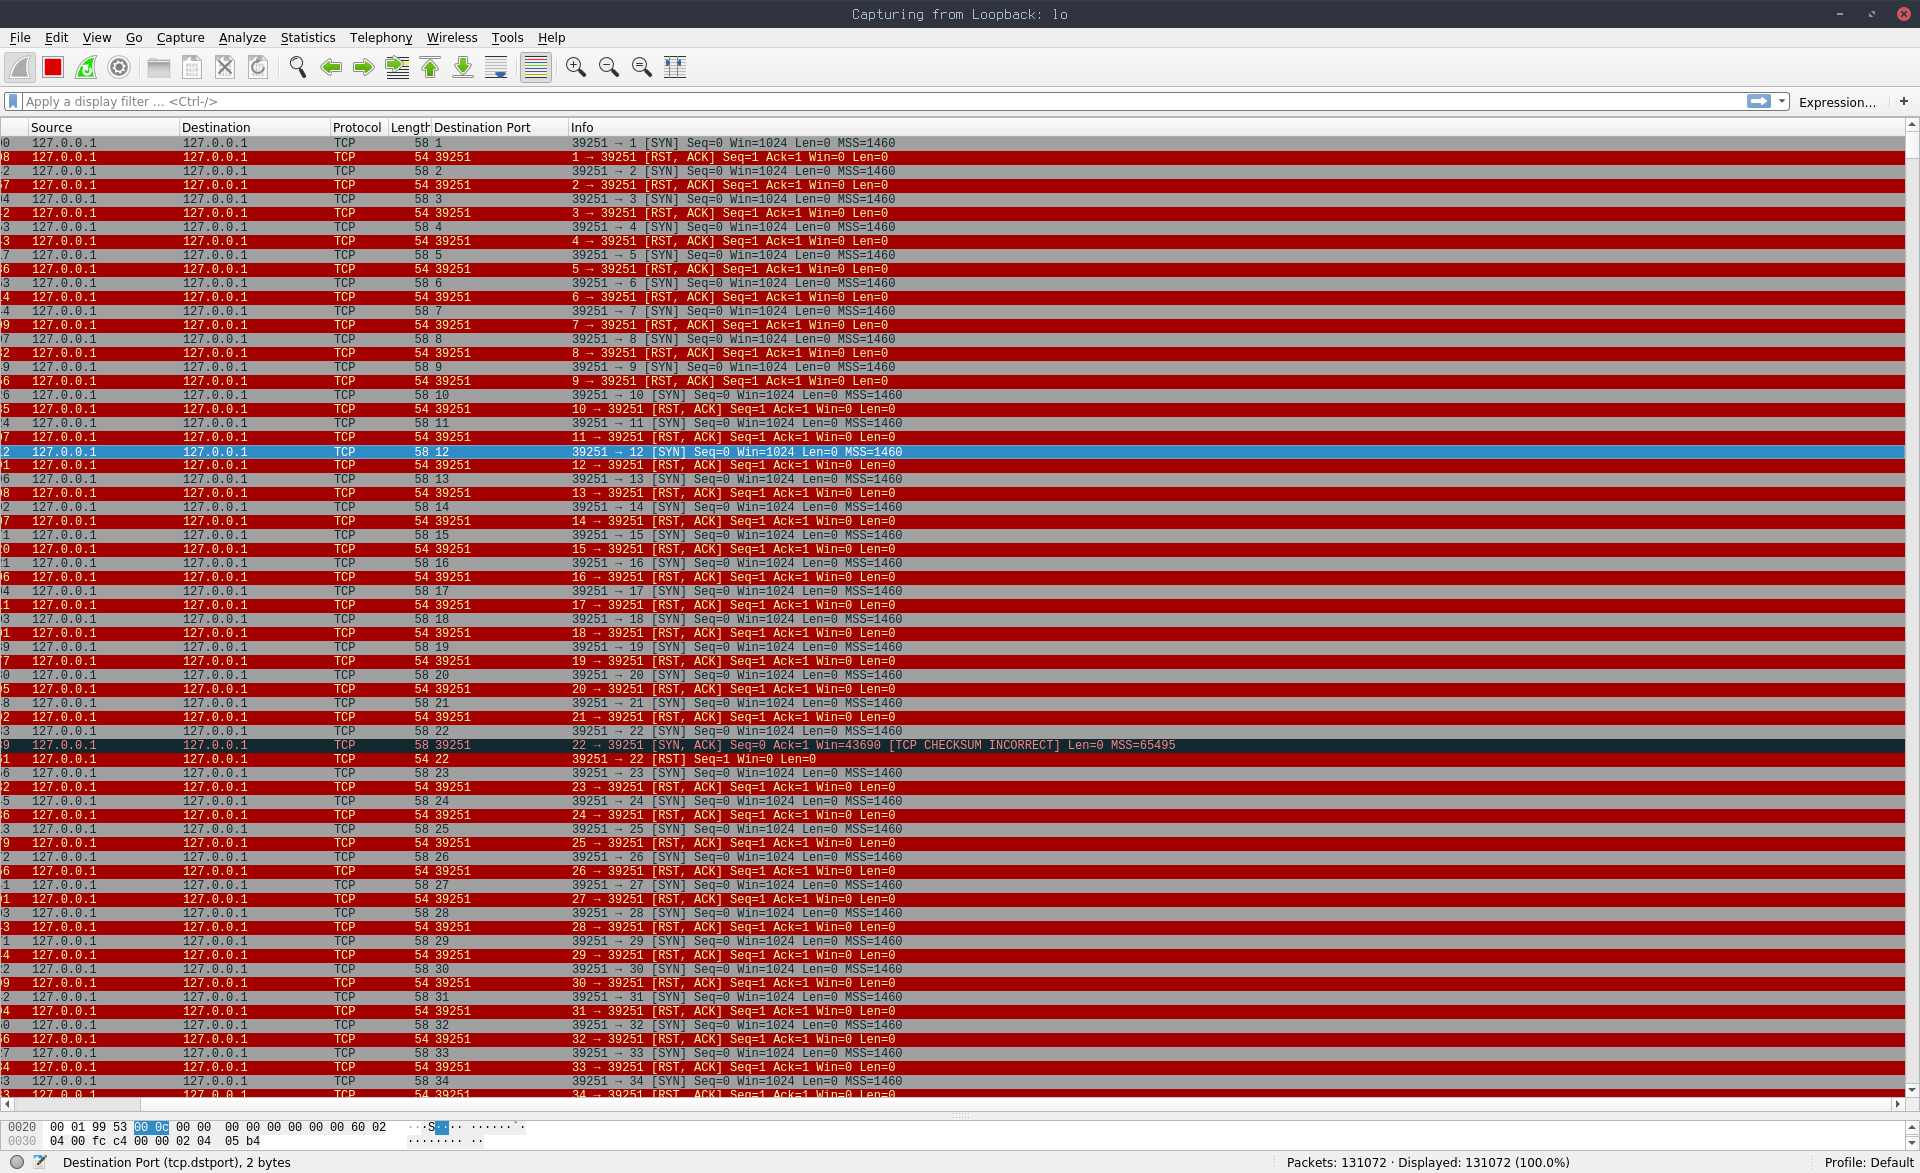
\includegraphics[width=\textwidth]{working_syn_full_scan.png}
  \caption{A fully working TCP-SYN scan.}
\end{figure}

\blindtext

\begin{figure}[h]
  \centering
  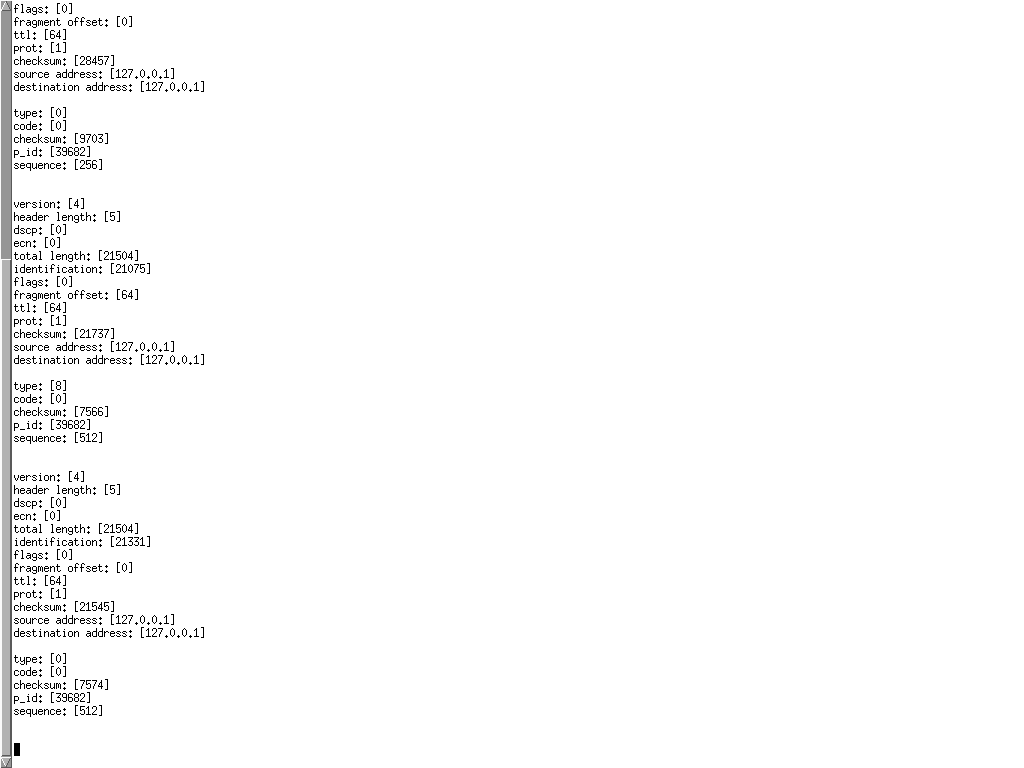
\includegraphics[width=\textwidth]{../screenshots/deconstructed_headers.png}
  \caption{IP headers deconstructed.}
\end{figure}

\blindtext
\blindtext
\blindtext

\end{document}
